\chapter{BAS-RELIEF BASED ON BRUSH STROKE }
Since the brush strokes can be extracted individually, it is natural to independently generate the individual depth maps and then merge the depth maps together to form the desired bas-relief, see Figure \ref{decom:overview}.It is noteworthy that a depth map can represent a bas-relief model.   In this Chapter, we demonstrate how to generate bas-relief surface from brush strokes, and how it can be modified. We also compare our algorithm against the two most notable 2D image based bas-relief generation algorithm. \\

 In our implementation, we employ the orthogonal SFS \cite{prados2004unifying} on the segmented strokes. These extracted strokes take into account the spatial occlusion and are suitable for manipulation. However, the SFS is performed on the opacity of the image rather than the intensity. The brightness equation used in SFS is expressed as,

\begin{equation*}
I(x)=\frac{1}{\sqrt{1+\lvert \bigtriangledown h \rvert ^2}}
\end{equation*}

It can be noted that the higher the intensity I, the smaller the change of depth h. Usually, some brush strokes tend to produce a high intensity in a painting. As a result, if the shape from shading algorithm is performed on intensity, the resulting stroke models will become flat and lack of hierarchy. Moreover, for a region, the boundary height is noticeably higher than its inside. This is because the gradient of the edges is always more than that of the inside. The opacity of image is independent of the color intensity (see Figure \ref{histo}). Each stroke has an appropriate distribution of opacity, which is in favor of a layered look, so we reformulate the equation : 
\begin{equation*}
\alpha(x)=\frac{1}{\sqrt{1+\lvert \bigtriangledown h \rvert ^2}}
\end{equation*}
$\alpha(x)$ is the opacity value of pixel $x$ on a brush stroke. 
To make the bas-relief more inflated,we rewrite the as,

\begin{equation}
\lVert \bigtriangledown h \rVert = \sqrt{\frac{1}{\lVert \alpha(x) \rVert ^2}-1+ \Delta}
\end{equation}
where $\Delta$ is a positive displacement. This modification may make the surface inflated. By solving this equation, we can generated a depth map for each brush stroke. As show in Figure \ref{strokerelief}, we input the opacity map of a decomposed layer, and from that layer we extract three brush strokes shown in different color,and by apply our algorithm we can generate bas-reliefs(depth maps) from each one of the brush strokes on this layers, and by generate bas-reliefs from all brush strokes, and merge them together, we automatically generate a bas-relief from the input Chinese painting. 
To differentiate the bas-relief generated form a single stroke and the final combined bas-relief, we use the term "stroke-relief" to indicate a bas-relief(depth map) generated from a single stroke. And just like a Chinese painting can be regarded as a union of brush strokes \cite{xu2006animating} ,in our approach, a bas-relief can be regarded as a union of stroke-relief.
\begin{figure}[H]
	\centering
	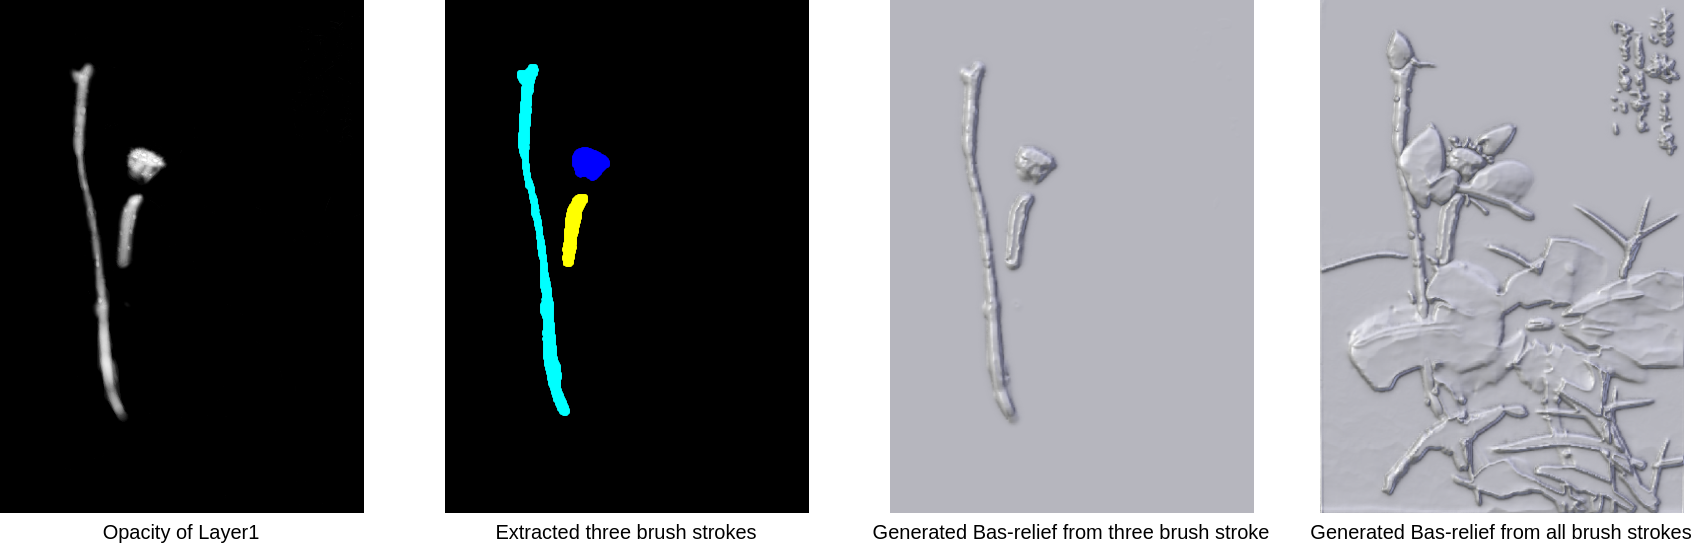
\includegraphics[width=15cm]{strokerelief.png}
	\caption{Bas-relief generation from brush strokes}
	\label{strokerelief}
\end{figure}



\section{Comparison}
This section compares our algorithm against the two most notable 2D image based bas-relief methods, 

The image-based bas-relief approaches\cite{zeng2014region} \cite{kolomenkin2011reconstruction} perform shape from shading algorithm separately on the segmented regions of an image.Most of segmentation methods work on image intensity. Due to lack of information of the spatial relationship, they always suffer from the issues of over-segmentation or incorrect segmentation. As a result, post-processing with user assistance to manipulate the depth maps is necessary. To illustrate this issue, we applied the  orthogonal SFS method \cite{prados2004unifying} on the segmented Rosemaling painting shown in Figure \ref{ETF} to generate the depth maps. It can be seen that there are lots of over-segmentation, or even incorrect segmentation as shown in Figure \ref{overseg}.


\section{Manipulate Bas-relief of stroke}

Moreover, it is desirable to allow the users to manipulate the brush stroke models for secondary creation purposes. We present three approaches based on the generated bar-relief models here.

\textbf{Rising a Stroke}  

For a set of stroke models, we may quantify their depth maps within a specified height scope. The order of strokes may be given by users. Suppose there are n overlapped strokes in a painting, which are sorted in a descending order from 1 to n. Let $S_i$ be the i-th stroke and $h_i(x)$ for the depth of point $x$ within $S_i$ . The depth map of $S_i$ is quantified within the scope of $[0,\rho]$ as,
\begin{equation}
h_i(x)= \frac{(\rho-(i-1)d)h_i(x)}{H_i}
\label{eq:raising}
\end{equation}

where $H_i=\frac{1}{\lvert S_i \rvert}\sum_{x\in S_i} h_i(x)  $, and d controls the depth difference between the successive order of stroke models. To manipulate stroke models, such as raising a stroke, this can be fulfilled by simply changing the order of  as shown in Figure \ref{raising}.
However, the scheme of Eq \ref{eq:raising} cannot settle the issue of two strokes obstructing each other. For example, stroke A partially obstructs the other stroke B while it may be partially obstructed by B. This can be resolved by the following stitching approach.\newline
\begin{figure}[H]
	\centering
	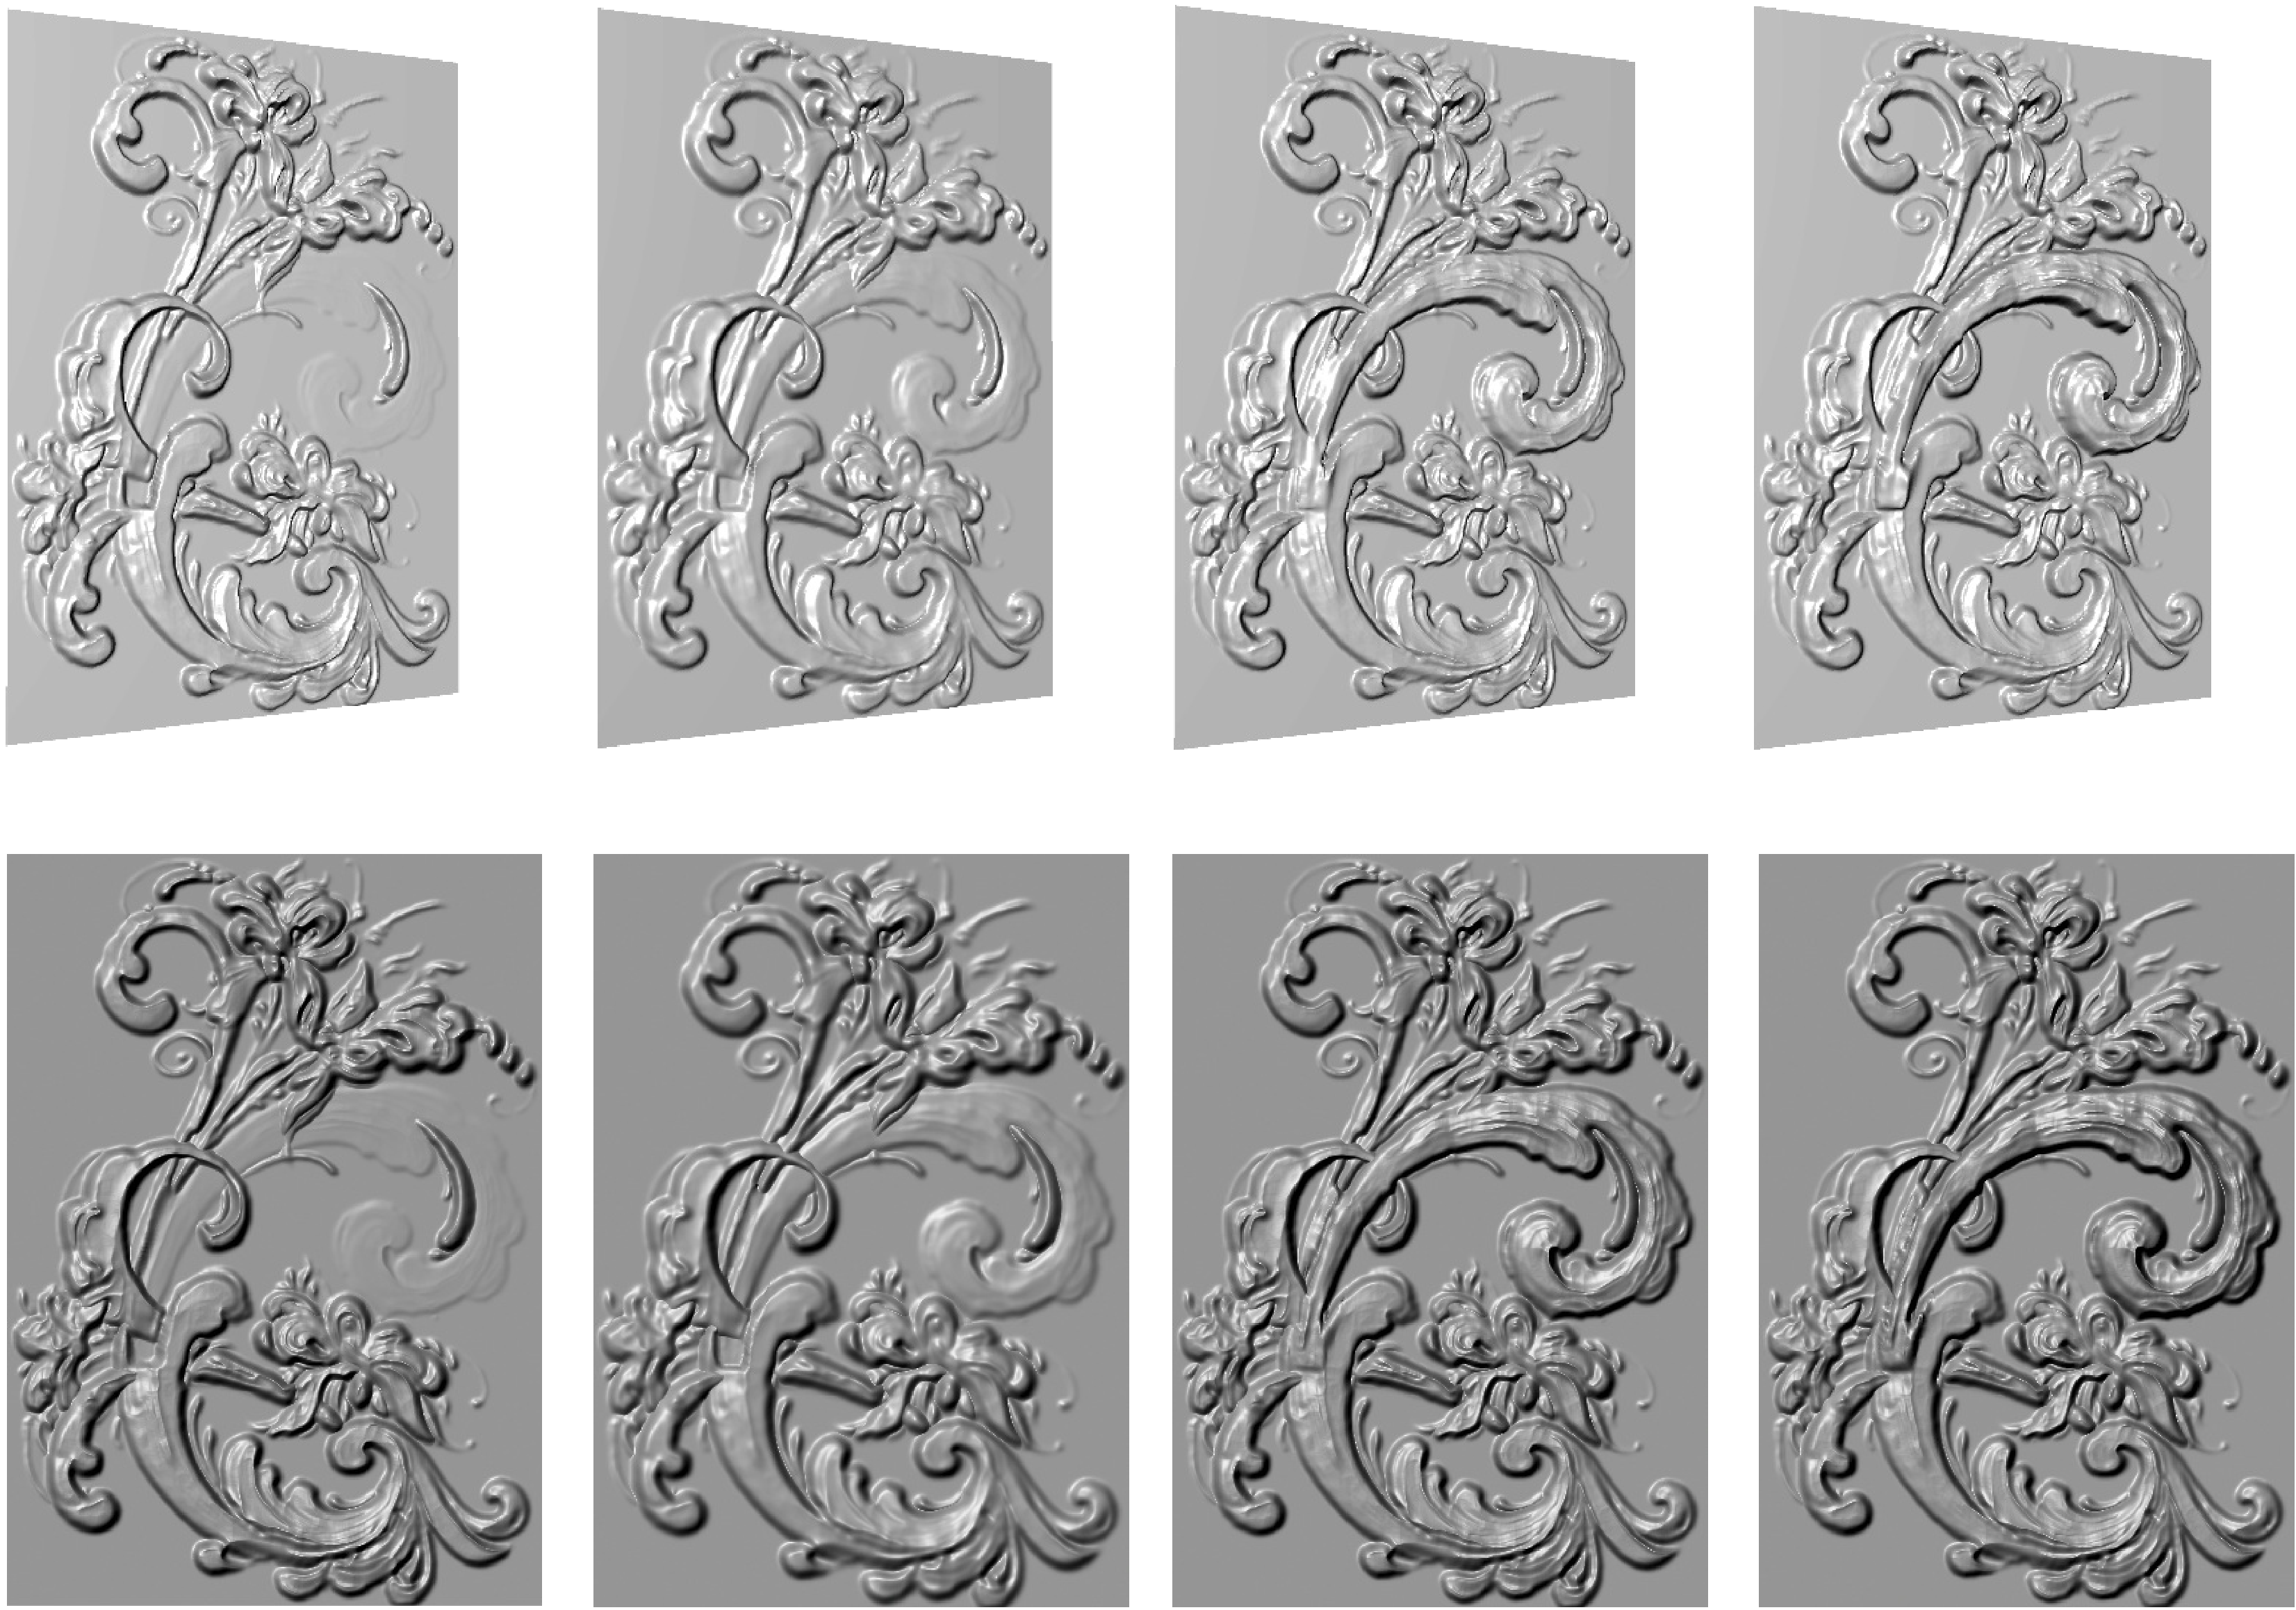
\includegraphics[width=15cm]{risestroke.png}
	\caption{Rising strokes}
	\label{raising}
	\medskip
	The selected strokes is rising from bottom to top in layer order. \\There are 4 layers.
\end{figure}

\textbf{Stitching one Stroke on Another one} 
\newline

For two overlapping strokes $S_i,S_j$, it is desired to stitch the model of $S_i$ on that of the other $S_j$ instead of overlapping their depth maps. This may be accomplished by solving for depth functions $h_i:S_i\rightarrow R $ such that the resulting $h_i$ satisfies stitching positional constraints. We define the set of $ D_{ij} \subseteq \partial S_i \cap \partial S_i $ as the stitching constraints. The depth functions are solved by minimizing the Dirichlet energy, 
\begin{equation}
 \int_{S_i} \lVert \bigtriangledown h_i - \vec{v_i} \rVert ^2 dx ,~ s.t. ~h_i(x)=h_j(x),\forall x \in D_{ij}
 \label{eq:stitch}
\end{equation}

where $\vec{v_i} $ denotes the differential coordinates of the model of $S_i$. Intuitively, this is to update $ h_i(x)$ which keeps close to the depth map of $S_i$ as much as possible while satisfying the positional constraints in a least squares sense. We perform the scheme of Eq \ref{eq:stitch} on the overlapping area of multiple strokes and illustrate all the possible spatial occlusion cases in Figure \ref{stitch}. It can be noted that there are four overlapped strokes to be depicted by using transparency in the Rosemaling painting. In fact there are at most eight occlusion cases as shown in Figure \ref{stitch}. We can further change the shape of these 3D strokes if needed.\newline

\begin{figure}[H]
	\centering
	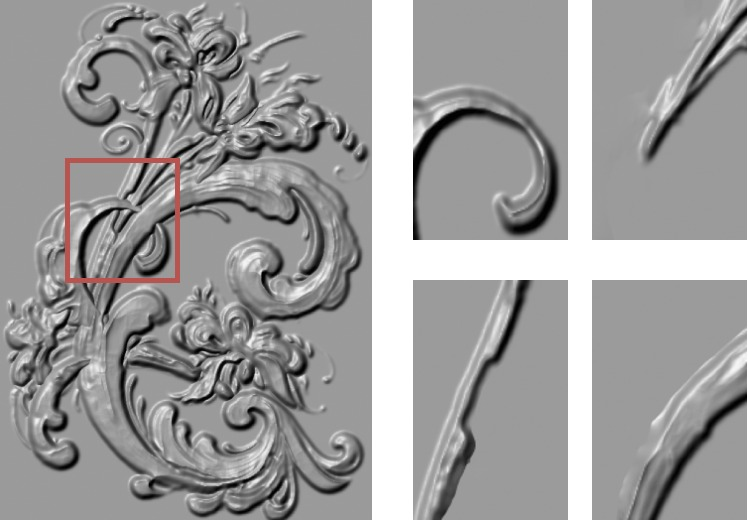
\includegraphics[width=14cm]{edit.jpg}
	\caption{Strokes segmented in selected region}
	\label{shape_edit}
\end{figure}

\begin{figure}[H]
	\centering
	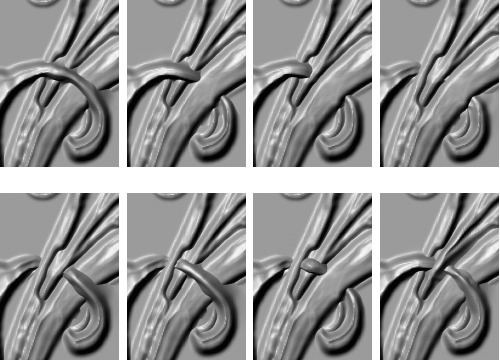
\includegraphics[width=14cm]{stitch.jpg}
	\caption{ The result of stitching strokes}
	\label{stitch}
	\medskip
 The result of stitching one stroke on another one. \\8 cases are highlighted by combining 4 selected strokes 
\end{figure}

\textbf{Changing the Shape of Strokes} 
\newline 

The key point is to determine the changed boundary of strokes on the background plane at first. For a given stroke $S_i$, the boundary of $S_i$ on the plane corresponds to the positional constraints in Eq \ref{eq:stitch}. When users change the boundary $\partial S_i $, the shape of the model of $S_i$ will be changed accordingly based on Eq \ref{eq:stitch}. Painters are used to sketching a skeleton $D_i^{'}$ on the background plane. It requires us to change the boundary of $S_i$ on the plane according to $D_i^{'}$.

To this end, $S_i$ is triangularized by a regular grid on the plane, and its skeleton may be extracted by the Hilditch thinning method \cite{cornea2007curve}. This skeleton can be matched to  $D_i^{'}$ by the lengths. The shape of boundary is deformed on the plane in terms of  $D_i^{'}$ . For an As-Rigid-As-Possible shape deformation \cite{weng20062d} on a plane, we employ the curve Laplacian coordinates on the boundary of $S_i$, $\lVert LV-\delta(V) \rVert ^2 $, where $V$ denotes the vertices of boundary $ \partial S_i $; the mean value coordinates $ \lVert MV \rVert^2 $, where $V$ denotes the vertices within $S_i$; and the positional constraints $D_i^{'}$, $\lVert CV-V^{'} \rVert ^2 $, where $V^{'} \in D_i^{'} $ while $V$ for the updated vertices. The boundary of $S_i$ is updated on the plane by minimizing the following sum of these three terms,

\begin{equation}
\lVert LV-\delta(V) \rVert ^2 + \lVert MV \rVert^2 + \lVert CV-V^{'} \rVert ^2 
\label{eq:shape_edit}
\end{equation}
 
Herein, we expand the matrices of $L,M,C$ through adding zero elements, such that V contains all the vertices of $S_i$ in Eq \ref{eq:shape_edit}. The resulting boundary of $S_i$ is then utilized in Eq \ref{eq:stitch} to update the depth functions of $S_i$ . Figure \ref{shape_edit} shows how to change the shape of the model of $S_i$. \newline 

\begin{figure}[H]
	\centering
	\begin{subfigure}[b]{0.3\textwidth}
		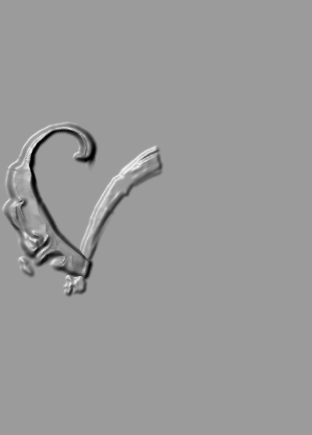
\includegraphics[width=\textwidth]{change.png}
		\caption{selected stroke}
		
	\end{subfigure}
	~  
	\begin{subfigure}[b]{0.3\textwidth}
		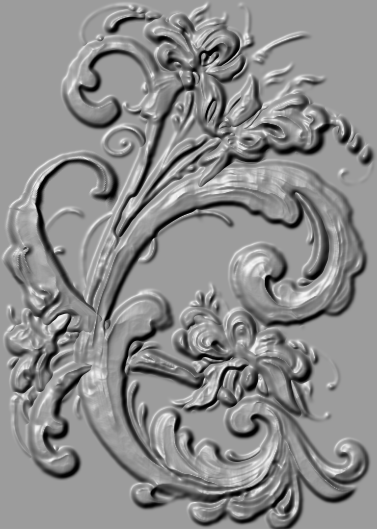
\includegraphics[width=\textwidth]{change1.png}
		\caption{modified depth map}
		
	\end{subfigure}
	\caption{The shape of a stroke is changed}
	\label{shape_edit}
\end{figure}

\textbf{Remark} Compared with image-based bas-relief generation, the main advantage of our approach is the introduction of “3D strokes”. Spatial occlusion offers an important cue in conveying the spatial relationship of the depicted objects and the depth information. Unlike the usual image segmentation problems, our method takes into account spatial occlusion in our stroke segmentation. As a result, over-segmentation and incorrect segmentation are largely eliminated. Moreover, the extracted “3D strokes” both help us sort out the stroke order and provide us a chance to rearrange the strokes as needed. This is in favor of further artistic creation in bas-relief design.

